\documentclass[journal]{IEEEtran}
\usepackage{amsmath,amssymb,booktabs,graphicx,multirow,url}
\usepackage[hidelinks]{hyperref}
\graphicspath{{results/figures/}}
% Auto-generated by proran.experiment; do not hand-edit.
\newcommand{\NoResHSR}{43.0}
\newcommand{\NoResQoS}{37.2}
\newcommand{\NoResWaste}{--}
\newcommand{\NoResOccupancy}{0.0}
\newcommand{\NoResLatency}{29.71}
\newcommand{\NoResP95Latency}{104.50}
\newcommand{\NoResBlock}{27.7}
\newcommand{\NoResEMBBQoS}{33.2}
\newcommand{\NoResURLLCQoS}{34.2}
\newcommand{\NoResMMTCQoS}{47.9}
\newcommand{\ReactiveHSR}{47.1}
\newcommand{\ReactiveQoS}{39.3}
\newcommand{\ReactiveWaste}{31.0}
\newcommand{\ReactiveOccupancy}{1.2}
\newcommand{\ReactiveLatency}{28.45}
\newcommand{\ReactiveP95Latency}{104.30}
\newcommand{\ReactiveBlock}{28.1}
\newcommand{\ReactiveEMBBQoS}{34.5}
\newcommand{\ReactiveURLLCQoS}{35.9}
\newcommand{\ReactiveMMTCQoS}{51.5}
\newcommand{\CertaintyHSR}{49.7}
\newcommand{\CertaintyQoS}{40.4}
\newcommand{\CertaintyWaste}{35.6}
\newcommand{\CertaintyOccupancy}{2.9}
\newcommand{\CertaintyLatency}{27.43}
\newcommand{\CertaintyP95Latency}{99.71}
\newcommand{\CertaintyBlock}{28.6}
\newcommand{\CertaintyEMBBQoS}{34.8}
\newcommand{\CertaintyURLLCQoS}{37.5}
\newcommand{\CertaintyMMTCQoS}{54.2}
\newcommand{\AwareHSR}{46.7}
\newcommand{\AwareQoS}{39.0}
\newcommand{\AwareWaste}{29.0}
\newcommand{\AwareOccupancy}{1.2}
\newcommand{\AwareLatency}{28.47}
\newcommand{\AwareP95Latency}{101.98}
\newcommand{\AwareBlock}{28.0}
\newcommand{\AwareEMBBQoS}{34.6}
\newcommand{\AwareURLLCQoS}{34.9}
\newcommand{\AwareMMTCQoS}{51.9}
\newcommand{\OracleHSR}{50.3}
\newcommand{\OracleQoS}{40.8}
\newcommand{\OracleWaste}{29.1}
\newcommand{\OracleOccupancy}{3.3}
\newcommand{\OracleLatency}{27.15}
\newcommand{\OracleP95Latency}{98.01}
\newcommand{\OracleBlock}{28.8}
\newcommand{\OracleEMBBQoS}{34.9}
\newcommand{\OracleURLLCQoS}{36.9}
\newcommand{\OracleMMTCQoS}{55.8}
\newcommand{\PPOHSR}{44.8}
\newcommand{\PPOQoS}{38.5}
\newcommand{\PPOWaste}{30.8}
\newcommand{\PPOOccupancy}{0.5}
\newcommand{\PPOLatency}{29.04}
\newcommand{\PPOP95Latency}{104.50}
\newcommand{\PPOBlock}{27.8}
\newcommand{\PPOEMBBQoS}{33.0}
\newcommand{\PPOURLLCQoS}{36.5}
\newcommand{\PPOMMTCQoS}{50.8}
\newcommand{\NoResHSRDiff}{+1.79}
\newcommand{\NoResHSRCILow}{+1.34}
\newcommand{\NoResHSRCIHigh}{+2.25}
\newcommand{\NoResQoSDiff}{+1.26}
\newcommand{\NoResQoSCILow}{+0.86}
\newcommand{\NoResQoSCIHigh}{+1.66}
\newcommand{\AwareHSRDiff}{-1.90}
\newcommand{\AwareHSRCILow}{-2.37}
\newcommand{\AwareHSRCIHigh}{-1.44}
\newcommand{\AwareQoSDiff}{-0.55}
\newcommand{\AwareQoSCILow}{-1.13}
\newcommand{\AwareQoSCIHigh}{+0.03}

% Auto-generated by web.scenario_audit; do not hand-edit.
\newcommand{\UrbanHSRGain}{+1.83}
\newcommand{\UrbanQoSGain}{+1.29}
\newcommand{\RushHSRGain}{+2.16}
\newcommand{\RushQoSGain}{+1.54}
\newcommand{\HighwayHSRGain}{+1.20}
\newcommand{\HighwayQoSGain}{+1.48}
\newcommand{\URLLCHSRGain}{+2.07}
\newcommand{\URLLCQoSGain}{+1.77}


\title{Uncertainty-Aware Proactive Resource Reservation for Network-Sliced 5G RAN Handovers}
\author{Reproducible Research Artifact}

\begin{document}
\maketitle

\begin{abstract}
Mobility can deliver a user equipment (UE) to a congested target cell before the scheduler can satisfy its slice service-level agreement (SLA). Reserving radio resource blocks (RBs) in advance can mitigate this risk, but inaccurate forecasts create waste and affect incumbent slices. We formulate reservation as a constrained sequential decision problem and evaluate a masked Proximal Policy Optimization (PPO) controller in a reproducible four-cell, three-slice simulator. A causal contract ledger enforces integer-RB capacity, activation, expiry, and wrong-target accounting, including simultaneous arrivals. The learned policy obtains \PPOQoS\% handover QoS satisfaction and \PPOHSR\% handover success at \PPOOccupancy\% reserved-RB occupancy, versus \NoResQoS\% and \NoResHSR\% without reservation; paired 95\% intervals exclude zero for both gains over no reservation. However, the uncertainty-aware heuristic exceeds PPO in handover success, and certainty-equivalent reservation exceeds both at a larger RB footprint. These synthetic results demonstrate a reliability--resource trade-off, not learned-policy dominance or field-network performance. Source code, tests, raw metrics, figures, and a live showcase accompany the paper.
\end{abstract}

\begin{IEEEkeywords}
5G, handover, network slicing, proactive reservation, prediction uncertainty, PPO, radio access network.
\end{IEEEkeywords}

\section{Introduction}
Network slicing multiplexes heterogeneous services over a shared radio access network (RAN).  eMBB seeks throughput, uRLLC emphasizes latency and reliability, and mMTC supports many modest-rate devices.  Mobility couples these requirements to a difficult admission-control problem: resources available in a serving cell say little about capacity at the target when handover completes.  Purely reactive control can be late, whereas blindly trusting a forecast reserves scarce capacity at the wrong cell or for too long.

PreNS combines attention-based bidirectional LSTM demand prediction with DDQN allocation and motivates confidence-aware predictive/reactive control~\cite{wu2026prens}.  Its published study, however, abstracts mobility and performs slice-level allocation rather than per-UE handover reservation.  Moreover, its printed confidence term has inverse-resource units while its variability term has squared metric units; adding them does not produce a dimensionally meaningful fusion weight.  We therefore retain the useful architectural premise but do not reproduce that fusion.

Related work addresses adjacent decisions: DeepCog forecasts cost-aware slice capacity~\cite{bega2020deepcog}; Li \emph{et al.} combine LSTM and advantage actor--critic for mobility-aware inter-slice allocation~\cite{li2020mobility}; and Gharehgoli \emph{et al.} study demand and channel-state uncertainty in end-to-end slicing~\cite{gharehgoli2023uncertainty}. Here the decision is instead a per-UE, target-cell RB hold with explicit timing, admission, consumption, and expiry. The comparison is methodological; our synthetic simulator does not reproduce those systems' evaluation settings.

This work contributes: (i) an explicit target/time/demand prediction contract; (ii) a causal integer-RB reservation ledger with wrong-target, early/late arrival, and activation-rejection semantics; (iii) a masked categorical PPO controller based on the clipped objective~\cite{schulman2017ppo} and generalized advantage estimation (GAE)~\cite{schulman2016gae}; and (iv) a reproducible evaluation with matched random traces, deterministic baselines, uncertainty sweeps, publication-quality plots, and a live simulator.

\section{System Model}
Let $i\in\mathcal U$, $j\in\mathcal C$, and $s(i)\in\{\mathrm{eMBB},\mathrm{uRLLC},\mathrm{mMTC}\}$ denote a UE, cell, and slice.  All RB counts refer to the same interval of duration $\Delta$.  Cell $j$ has integer capacity $K_j$, incumbent allocation $A_{j,t}$, and active per-UE reservations $B_{i,j,t}$.  The fundamental invariant is
\begin{equation}
A_{j,t}+\sum_i B_{i,j,t}\le K_j, \qquad
F_{j,t}=K_j-A_{j,t}-\sum_iB_{i,j,t}\ge0. \label{eq:capacity}
\end{equation}
The simulator uses strict-priority admission (uRLLC, eMBB, mMTC) only to produce a controlled congestion process; it does not claim to model a production NR scheduler.  Each UE has minimum $d_i^{\rm SLA}$ RBs and slice latency bound $L_{s(i)}^{\max}$.  SLA satisfaction is evaluated after handover and never asserted when the physical capacity is infeasible.

At decision time, projected kinematics select one candidate target $j$ within horizon $H$. The synthetic forecaster exposes a heuristic score $p_{i,j,t}\in[0,1]$, relative arrival lead $\hat h_{i,j,t}\in\{1,\ldots,H\}$, and estimated RB demand $\hat D_{i,j,t}$. The score is an input to the controller, not a calibrated conditional probability or a multi-target distribution. Forecast perturbations generate reproducible nonstationary errors. The state separately includes a configured target-noise rate $u^T\in[0,1]$ and capacity-normalized deviation from the currently observed demand $u^D\ge0$. Neither is evidence of a fitted uncertainty estimator.

\section{Reservation MDP}
An action is $a_t=(b_t,q_t,d_t)$, where $b_t$ selects reservation, $q_t$ is an integer amount, and $d_t$ is activation delay.  Positive actions obey
\begin{equation}
1\le q_t\le\hat D_{i,j,t},\qquad 0\le d_t\le\hat h_{i,j,t}. \label{eq:action}
\end{equation}
The implementation enumerates no-op plus half/full demand at immediate, midpoint, and just-in-time activation.  A deterministic mask removes actions violating (\ref{eq:action}) or known commitments; no-op is always legal.  Runtime activation rechecks (\ref{eq:capacity}).  A contract remains active until the first next handover or expiry $t+H$.  Early arrival cannot use an inactive promise; wrong-target and expired active contracts count as unused.

For a realized handover with demand $D_i$, matching held reservation $B_i^{-}$ and free RBs $F_i^{-}$, serviceable capacity and used reservation are
\begin{equation}
X_i=\min(D_i,B_i^{-}+F_i^{-}),\qquad
U_i=Y_i^{\rm HO}\min(D_i,B_i^{-}), \label{eq:handover}
\end{equation}
where $Y_i^{\rm HO}$ is the observed success flag.  This prevents a failed or wrong-target handover from retroactively ``using'' reserved RBs.

The normalized interval reward is
\begin{equation}
r_t=\alpha h_t+\beta q_t^{\rm QoS}-\gamma\frac{W_t}{\sum_jK_j}
-\delta\frac{\sum_{i,j}B_{i,j,t}}{\sum_jK_j}, \label{eq:reward}
\end{equation}
where $h_t$ and $q_t^{\rm QoS}$ are event success fractions, and $W_t$ is unused activated RBs resolved in the interval.  We use $(\alpha,\beta,\gamma,\delta)=(2,3,1.5,0.25)$.

The state contains forecast score $p$, normalized time-to-handover, predicted demand and free RBs, target load, $u^T$, $u^D$, one-hot slice, normalized SLA RBs/latency, speed, and bias. For legal action set $\mathcal A(s)$, the masked policy is
\begin{equation}
\pi_\theta(a|s)=\frac{\exp \ell_\theta(s,a)}{\sum_{a'\in\mathcal A(s)}\exp\ell_\theta(s,a')},\quad a\in\mathcal A(s), \label{eq:masked}
\end{equation}
and zero otherwise.  The saved rollout mask is reused during updates.  With TD residual $\delta_t^{V}=r_t+\gamma_{\rm RL}(1-d_t)V(s_{t+1})-V(s_t)$, GAE computes $\hat A_t=\sum_{k\ge0}(\gamma_{\rm RL}\lambda)^k\delta_{t+k}^{V}$ up to termination.  PPO maximizes the standard clipped likelihood-ratio surrogate~\cite{schulman2017ppo}.  A linear actor/critic is deliberately used: it is inspectable, sufficient for the normalized state, and makes the artifact runnable on a CPU without a deep-learning framework.

\section{Experimental Method}
The simulated $100\times100$~m area contains four nearest-cell regions, 32 moving UEs, and 60 RBs per cell. Velocities undergo bounded Gaussian perturbations; traffic has a shared periodic component, slice-specific Gaussian demand, and bursty uRLLC demand. The horizon is eight 100-ms intervals. Mean demands are 10.5, 7.0, and 3.2 RBs; SLA floors are 7, 5, and 2 RBs for eMBB, uRLLC, and mMTC. These are declared simulation assumptions, not 3GPP-calibrated deployment values.

The actor is first behavior-cloned~\cite{pomerleau1989alvinn} from the uncertainty-aware heuristic on 12 independent episodes. No-op examples are capped at twice the positive reservation examples. After 45 categorical-likelihood epochs, PPO fine-tunes for 60 episodes of 180 intervals with $\gamma_{\rm RL}=0.985$, $\lambda=0.95$, clip 0.2, six epochs per rollout, and fixed seed 41. Evaluation uses 20 disjoint seeds, 320 intervals each. Every method receives identically seeded mobility, traffic, and radio random streams. Baselines are: no reservation; reactive full reservation one interval before forecast arrival; certainty-equivalent immediate full reservation above score 0.42; the uncertainty-aware teacher; and a privileged projection reference that knows whether the noisy target equals the unperturbed kinematic projection. The reference does not know realized future mobility or congestion and is not an achievable operational method.

Metrics follow RB-consistent denominators: handover success rate (HSR), QoS satisfaction, unused activated-RB fraction, time-average reservation occupancy, incumbent block rate, and modeled event-latency CDFs separated by slice. The latency proxy includes both successful and failed attempts; QoS satisfaction requires a successful handover, full demand, and a latency below the slice bound. Undefined denominators are reported as such; no reservation therefore has no waste percentage. Because every method uses the same 20 seeds, controller differences are analyzed per seed with two-sided 95\% paired $t$ intervals ($t_{0.975,19}=2.093$).

\section{Results}
\begin{table}[t]
\centering
\caption{Matched-seed test performance (20 runs). Percent except latency.}
\label{tab:main}
\resizebox{\columnwidth}{!}{%
\begin{tabular}{lrrrrr}
\toprule
Method & HSR & QoS & Waste & Occup. & Mean ms\\
\midrule
No reservation & \NoResHSR & \NoResQoS & -- & \NoResOccupancy & \NoResLatency\\
Reactive & \ReactiveHSR & \ReactiveQoS & \ReactiveWaste & \ReactiveOccupancy & \ReactiveLatency\\
Certainty-equivalent & \CertaintyHSR & \CertaintyQoS & \CertaintyWaste & \CertaintyOccupancy & \CertaintyLatency\\
Uncertainty-aware & \AwareHSR & \AwareQoS & \AwareWaste & \AwareOccupancy & \AwareLatency\\
Projection reference & \OracleHSR & \OracleQoS & \OracleWaste & \OracleOccupancy & \OracleLatency\\
PPO (proposed) & \PPOHSR & \PPOQoS & \PPOWaste & \PPOOccupancy & \PPOLatency\\
\bottomrule
\end{tabular}}
\end{table}

\begin{table}[t]
\centering
\caption{Per-slice handover QoS satisfaction (\%); mean across 20 test seeds.}
\label{tab:slices}
\begin{tabular}{lrr}
\toprule
Slice & No reservation & PPO\\
\midrule
eMBB & \NoResEMBBQoS & \PPOEMBBQoS\\
uRLLC & \NoResURLLCQoS & \PPOURLLCQoS\\
mMTC & \NoResMMTCQoS & \PPOMMTCQoS\\
\bottomrule
\end{tabular}
\end{table}

Table~\ref{tab:main} shows PPO at \PPOQoS\% QoS and \PPOHSR\% HSR, compared with \NoResQoS\% and \NoResHSR\% without reservation. The paired PPO-minus-baseline differences are \NoResQoSDiff\ percentage points QoS (95\% CI $[\NoResQoSCILow,\NoResQoSCIHigh]$) and \NoResHSRDiff\ points HSR (CI $[\NoResHSRCILow,\NoResHSRCIHigh]$). Relative to the uncertainty-aware heuristic, the differences are \AwareHSRDiff\ points HSR (CI $[\AwareHSRCILow,\AwareHSRCIHigh]$) and \AwareQoSDiff\ points QoS (CI $[\AwareQoSCILow,\AwareQoSCIHigh]$). PPO uses less reservation occupancy (\PPOOccupancy\% versus \AwareOccupancy\%) but has slightly more unused activated RBs (\PPOWaste\% versus \AwareWaste\%). Certainty-equivalent reservation reaches \CertaintyHSR\% HSR at \CertaintyOccupancy\% occupancy, while the privileged projection reference reaches \OracleHSR\%. Blocking is \PPOBlock\% for PPO versus \NoResBlock\% without reservation. Thus PPO improves the no-reservation outcome but does not dominate simpler policies.

Table~\ref{tab:slices} exposes eMBB, uRLLC, and mMTC handover QoS outcomes separately. PPO improves the latter two but slightly reduces eMBB QoS on this test suite. The priority scheduler differentiates admission order, but these rates are measured outcomes under shared finite capacity, not a proof of hard slice isolation.

\begin{figure}[t]
\centering
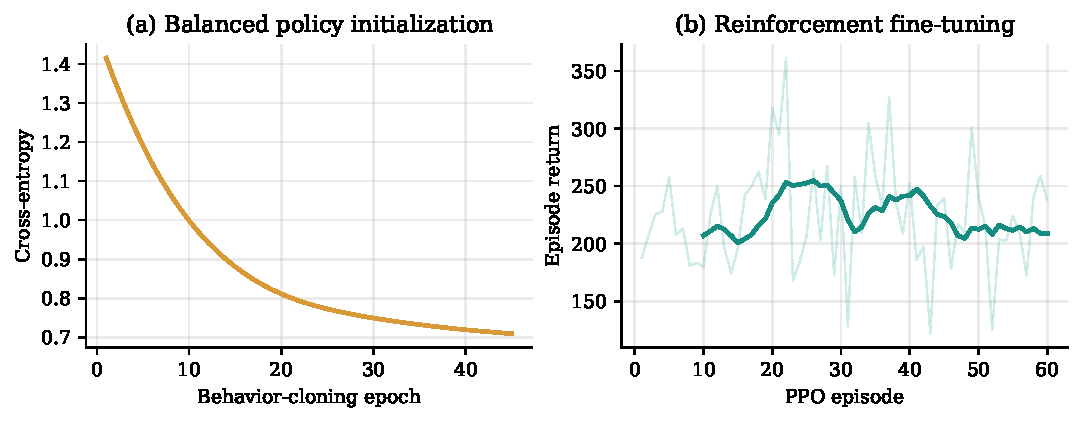
\includegraphics[width=\columnwidth]{learning_stages.pdf}
\caption{Two-stage learning: balanced behavior-cloning initialization followed by PPO reinforcement fine-tuning.}
\label{fig:training}
\end{figure}

Figure~\ref{fig:training} records the actual PPO optimization trace; a separate behavior-cloning loss is retained in the artifact. Figure~\ref{fig:pareto} sweeps a deterministic reliability threshold and overlays learned and baseline policies. PPO occupies less RB-time than the teacher but loses HSR and QoS; certainty-equivalent reservation yields higher HSR and QoS at higher occupancy. The full frontier prevents a single favorable metric from hiding this trade-off.

An exploratory, post-training stress audit applies the saved PPO actor to four frozen workloads on eight matched seeds each, with 240 intervals per seed. These workloads are independent of the six-device educational web traces. Mean PPO-minus-no-reservation HSR differences are $\UrbanHSRGain$, $\RushHSRGain$, $\HighwayHSRGain$, and $\URLLCHSRGain$ percentage points for urban, rush-hour, highway, and elevated-uRLLC-burst settings, respectively; the corresponding QoS differences are $\UrbanQoSGain$, $\RushQoSGain$, $\HighwayQoSGain$, and $\URLLCQoSGain$ points. The workloads alter UE density, capacity, speed, or burst rate, but do not change the underlying mobility or radio abstraction. These small-sample checks are directional robustness evidence, not deployment validation or a model-selection set. Per-seed values are supplied in \texttt{scenario\_audit.csv}.

\begin{figure}[t]
\centering
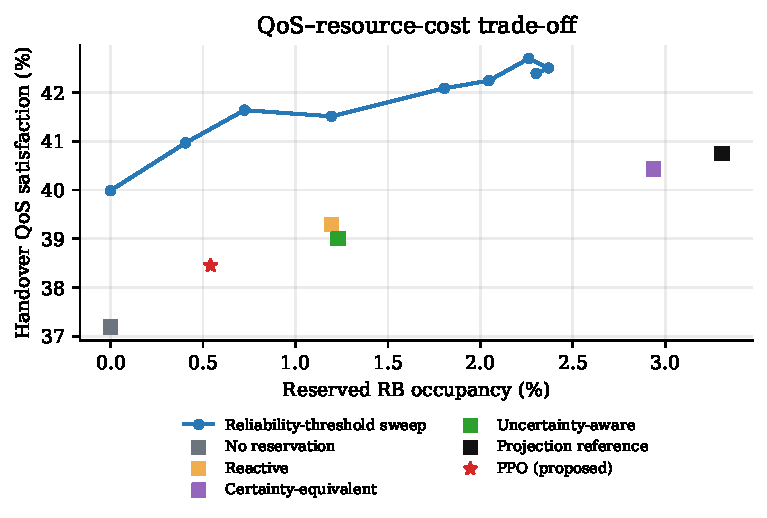
\includegraphics[width=.95\columnwidth]{qos_resource_pareto.pdf}
\caption{Handover QoS versus time-average reserved-RB occupancy.}
\label{fig:pareto}
\end{figure}

\begin{figure*}[t]
\centering
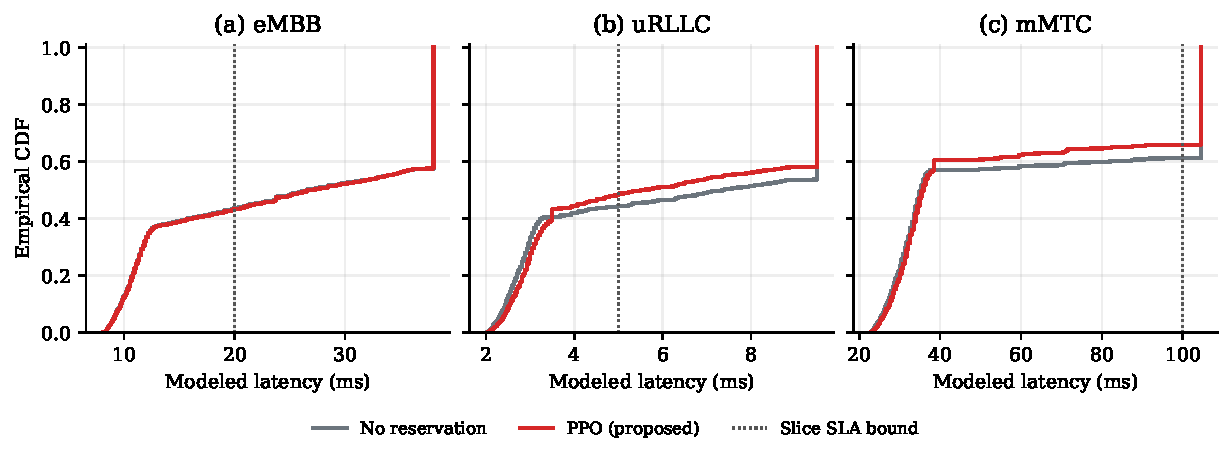
\includegraphics[width=.92\textwidth]{slice_latency_cdf.pdf}
\caption{Modeled latency CDF by slice for no reservation and PPO; dotted vertical lines show each slice's configured latency bound. All attempted handovers are included.}
\label{fig:cdf}
\end{figure*}

The aggregate mean modeled latency is \PPOLatency~ms for PPO and \NoResLatency~ms without reservation; Fig.~\ref{fig:cdf} separates the three slice distributions. Reservation is an admission mechanism, not a latency cure: when a handover remains demand-limited, the synthetic shortfall penalty dominates. Per-slice calibration against a link/system-level simulator is required before operational conclusions.

\section{Validity, Reproducibility, and Limitations}
Capacity is asserted after every handover and interval in unit tests, including simultaneous arrivals at one cell. Other tests cover no-op feasibility, action bounds, deterministic matched traces, undefined zero-denominator metrics, masked probabilities, and finite PPO updates. Raw per-method means and standard deviations are retained in CSV/JSON. A web dashboard exposes UE motion, slice classes, contracts, clickable RB ledgers, and handover outcomes.

The experiment is synthetic. It abstracts channel quality, beam failure, signaling delay, HARQ, a standards-compliant scheduler, and per-slice hard isolation. The predictor is controlled stochastic kinematics with an uncalibrated score, not a fitted model. The serialized one-candidate decision rule limits controller throughput, and the linear PPO policy is intentionally small. Icons for cars, drones, and robots are illustrative; they share the same mobility model. Consequently, the numerical results establish internal algorithmic behavior and reproducibility, not deployment performance. Future work should fit calibrated predictors, evaluate across more seeds and scenarios, include realistic NR link adaptation, and test multi-candidate control~\cite{li2020mobility,gharehgoli2023uncertainty}.

\section{Conclusion}
We developed a complete uncertainty-aware proactive reservation artifact for sliced 5G handovers.  Its central design choice is to preserve uncertainty as observable error while enforcing capacity through a causal contract ledger and a masked PPO action space.  Experiments show modest QoS/reliability gains with measurable occupancy, waste, and blocking costs.  The absence of uniform dominance is itself informative: proactive reservation should be selected from an explicit reliability--efficiency frontier, not justified by a single aggregate score.

\bibliographystyle{IEEEtran}
\bibliography{references}
\end{document}
